\section{Illustration de la criticité du problème de mobilité dans la ville de Yaoundé}

Essayons de voir à quel point le problème de la mobilité dans la ville de Yaoundé, est alarmant.

Tout d'abord, d'un point de vue général, le domaine du transport est un domaine crucial dans la vie d'un pays, tant il impacte son économie, la vie de ses citoyens et l'environnement (pollution important en cas d'embouteillages). 

Pour mieux cerner ces impacts, réalisons que une étude montre qu'un habitant de Yaoundé passe en moyenne 30 minutes dans les embouteillages \cite{mfoulou2016mobilite}. Bien plus, le gouvernement se voit contraint à cause de ces congestion à débourser des milliards de FCFA chaque année pour créer d'autres alternatives routières.\cite{237online2022contournement}

Terminons par un exemple palpable: Considérons la multitude des étudiants qui vivent dans les quartiers périphériques de Yaoundé (Emana, Nkoabang, Odja, Nkolbissong) et qui doivent se rendre tous les matins à l'ENSPY\footnote{École Nationale Supérieure Polytechnique de Yaoundé} où les cours débutent en majorité à 7h30. Ces derniers se retrouvent à passer 30 à 45 min au moins dans les embouteillages comme ceux de la figure \ref{fig:embouteillage}, et très souvent sont fréquemment en retard aux premières heures de cours. Pire encore, les cours finissant entre 17h et 18h, ces derniers, toujours à cause des congestions, arrivent chez eux pas moins avant 19h, fatigués d'avoir traînés dans les embouteillages. C'est ainsi qu'ils n'ont presque pas de temps pour réviser les leçons de la journée.

\begin{figure}[h]
    \centering
    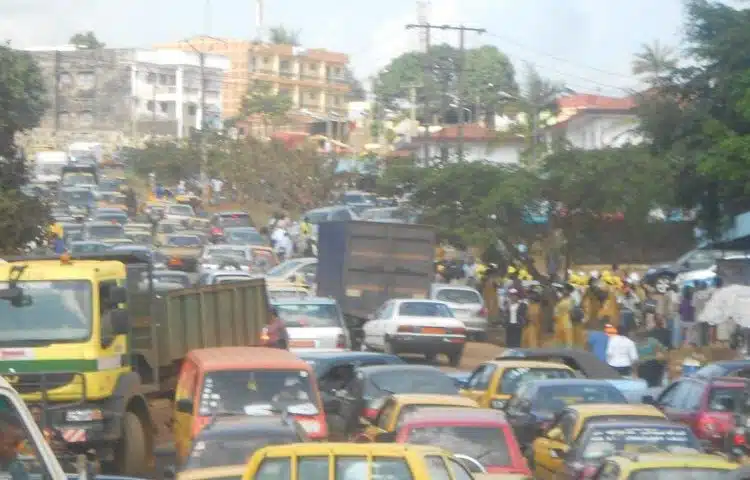
\includegraphics[width=0.5\linewidth]{Images/Embouteillage.png}
    \caption{Embouteillages - Yaoundé}
    \label{fig:embouteillage}
    \cite{camerounCirculation}
\end{figure}

Or une plate-forme permettant au conducteurs de s'orienter dans les directions optimales pour équilibrer le flux de circulation et par ce fait leur temps de trajet, ferait bien l'affaire de ces étudiants et des citoyens de Yaoundé en général, voir des grandes villes du monde.

Analysons maintenant les corrélations d'une telle solution avec les acteurs déjà présents dans le société.